%!TEX program = xelatex
% HUSTthesis.tex @ https://github.com/zfengg/HUSTtex/tree/master/HUSTthesis
%
% 	A simple tex template for the undergraduate thesis at HUST.
%
% author: Zhou Feng @ 2019
%
% requirements:
%	TeX environments: TeXlive/MacTeX or MiKTeX
%	compiler: XeLaTeX
%
% ---------------------------------------------------------------------------- %
%                                   preamble                                   %
% ---------------------------------------------------------------------------- %
\documentclass[a4paper]{article}
% 10.5pt = 5 hao

% ---------------------------------- layout ---------------------------------- %
\usepackage[a4paper,top=2.5cm,bottom=2.5cm,left=3cm,right=3cm,% margins
			headheight=1.5cm,headsep=1.5em,
			footskip=2em,
			]{geometry}

% ------------------------------- math symbols ------------------------------- %
% 载入常用的数学包, 符号包
\usepackage{amsmath}
\usepackage{amsfonts}
\usepackage{amssymb}
\usepackage{mathrsfs}
\usepackage{blindtext}
\usepackage{tikz}

%----------------------------------------------------------------%
%% linespace 行间距,段间距等等
\usepackage{setspace}
% \usepackage{indentfirst} % then the first line of each title should start with a indent.
% 定义标题和段落样式
% 定义1.5倍行距
\renewcommand{\baselinestretch}{1.62}
\setlength{\baselineskip}{12pt}   % set the fixed value of the lineskip
\setlength\parskip{\baselineskip} % set the space between the paragraphs, set the variable \parskip \baselineskip
% parindent
\setlength{\parindent}{0pt}

%----------------------------------------------------------------%
% fonts (style, color, size). 字体的大小,颜色,以及定义常用的字号
\usepackage{ctex}		 	% If you are lazy, the CTEX suit is enough.
% Chinese font
\usepackage{xeCJK}		 	% For the Chinese through XeLaTex
\setCJKmainfont{FandolSong} 	% set the mainfont of Chinese as songti. (serif) for  
\setCJKsansfont{FandolSong}	% sans serif font for \textsf
\setCJKmonofont{FandolSong}	% monospace font for \texttt
% \punctstyle{kaiming}   	% Remove the space used by symbols like comma. Special for the mainland students like us HUSTers.
\setCJKfamilyfont{song}{FandolSong}                     %宋体 song
\newcommand{\song}{\CJKfamily{song}}                        
\setCJKfamilyfont{kai}{FandolKai}                        		 %楷体2312  kai
\newcommand{\kai}{\CJKfamily{kai}}  
\setCJKfamilyfont{hwzs}{FandolFang}                        %华文中宋  hwzs
\newcommand{\hwzs}{\CJKfamily{hwzs}}
\setCJKfamilyfont{hei}{FandolHei}                     %黑体  hei
\newcommand{\hei}{\CJKfamily{hei}}
% English font
\usepackage{fontspec}% Then you can use the fonts installed at your device.
\setmainfont{Times New Roman}
\setsansfont{Times New Roman}
\setmonofont{Times New Roman}
%\setsansfont{[foo.ttf]} % for the fonts at this default path.
% font Color 利用definecolor自己可以定义颜色
\usepackage{xcolor}
\definecolor{MSBlue}{rgb}{.204,.353,.541}
\definecolor{MSLightBlue}{rgb}{.31,.506,.741}
% font Size (I use pinyin represents the corresponding size in Microsorft Word)
% \newcommand{\chuhao}{\fontsize{42pt}{\baselineskip}\selectfont}
\newcommand{\xiaochuhao}{\fontsize{36pt}{\baselineskip}\selectfont}
% \newcommand{\yihao}{\fontsize{28pt}{\baselineskip}\selectfont}
\newcommand{\erhao}{\fontsize{21pt}{\baselineskip}\selectfont}
\newcommand{\xiaoerhao}{\fontsize{18pt}{\baselineskip}\selectfont}
\newcommand{\sanhao}{\fontsize{15.75pt}{\baselineskip}\selectfont}
\newcommand{\sihao}{\fontsize{14pt}{18pt}\selectfont}
\newcommand{\xiaosihao}{\fontsize{12pt}{18pt}\selectfont}
\newcommand{\wuhao}{\fontsize{10.5pt}{18pt}\selectfont}
% \newcommand{\xiaowuhao}{\fontsize{9pt}{\baselineskip}\selectfont}
% \newcommand{\liuhao}{\fontsize{7.875pt}{\baselineskip}\selectfont}
% \newcommand{\qihao}{\fontsize{5.25pt}{\baselineskip}\selectfont}

% ---------------------------------------------------------------------------- %
%% header and footer 页眉,页脚
\usepackage{fancyhdr} % for header and footer
% 设置页眉样式
\newcommand{\headstyle}{
 \fancyhead[C]{ \hwzs\wuhao 华\hspace{0.5em}中\hspace{0.5em}科\hspace{0.5em}技\hspace{0.5em}大\hspace{0.5em}学\hspace{0.5em}本\hspace{0.5em}科\hspace{0.5em}生\hspace{0.5em}结\hspace{0.5em}课\hspace{0.5em}论\hspace{0.5em}文\hspace{0.5em}}
}
% 设置页脚样式
\newcommand{\footstyle}{\fancyfoot[C]{\wuhao\thepage}
 \fancyfoot[L]{\rule[5pt]{6.7cm}{0.4pt}}
 \fancyfoot[R]{\rule[5pt]{6.7cm}{0.4pt}}
}
\pagestyle{fancy}
\fancyhf{} % 清空原有样式
\headstyle
\footstyle
% 定义一种新的格式叫做main
\fancypagestyle{main}{%
 \fancyhf{} % 清空原有样式
 \headstyle
 \footstyle
}
\renewcommand{\headrulewidth}{0.4pt}
% \renewcommand{\footrulewidth}{0.4pt}
% \renewcommand{\headrule}{\rule{\textwidth}{0.4pt}}

% ---------------------------------------------------------------------------- %
% set the styles of sections at all levels
% 设置各个标题样式
% 不需要使用part和chapter层级
\usepackage{titlesec}
\usepackage{titletoc}
\titleformat{\section}{\centering\hei\bfseries\xiaoerhao}{\thesection}{1em}{} % 在section标题编号后面加个点
% \titlelabel{\thetitle.\quad} % add a dot after the counter for all levels of sections
% \titleformat*{\section}{\wuhao\bfseries} % 设置标签的形式,5号加粗
\titleformat*{\subsection}{\raggedright\hei\bfseries\sihao}
\titleformat*{\subsubsection}{\raggedright\hei\bfseries\xiaosihao}
\titleformat{\paragraph}[hang]{\raggedright\hei\bfseries\xiaosihao}{\theparagraph}{1em}{}[]

% manual
% \titleformat{command}[shape]{format}{label}{sep}{before-code}[after-code]
% \titlespacing{command}{left}{before-sep}{after-sep}
% 设置新的层级subsubsubsection
\setcounter{tocdepth}{4}
\setcounter{secnumdepth}{4}

\newcommand{\sectionbreak}{\clearpage} % 小节从新的一页开始
% 根据学校要求设置新的section, subsection, subsection,  paragraph

% set the content of section and so on
\newcommand\seccontent{
	\song
	\xiaosihao % 默认五号字体, 行间距为1.5*\baselineskip
    \setlength{\parindent}{2em} % 首段缩进两个M字符
    \setlength{\parskip}{0pt}
    }
\newcommand\tabcontent{
	\song
	\wuhao % 默认五号字体, 行间距为1.5*\baselineskip
	\setlength{\parindent}{2em} % 首段缩进两个M字符
	\setlength{\parskip}{0pt}
}


% ---------------------------------------------------------------------------- %
% for the style of theorems, definitions, proofs and remarks 定义数学里面一些常用的环境
\usepackage{amsthm}
\newtheorem{thm}{\textbf{定理}}[section]
% The section in [] can be replaced by chapter or subsection
\theoremstyle{definition} 
\theoremstyle{plain}
\theoremstyle{remark}

% ---------------------------------------------------------------------------- %
% for the caption and reference 图表及公式的编号规范
\usepackage{float} 		 		  	% table figure positioning
\usepackage{caption}
\captionsetup[figure]{labelformat=default, labelsep=quad,name={图}}
\captionsetup[table]{labelformat=default,labelsep=quad,name={表}}
% 设置图表标题的计数方式
\renewcommand{\thefigure}{\ifnum \thesection>0 \thesection-\fi \arabic{figure}} % set caption label style to 2-1
\renewcommand{\thetable}{\ifnum \thesection>0 \thesection-\fi \arabic{table}} % set caption label style to 2-1
\DeclareCaptionFont{mylabelfont}{\hei\xiaosihao}
\captionsetup[figure]{font=mylabelfont}
\captionsetup[table]{font=mylabelfont}

% 设置图表的autoref的格式
\newcommand{\reffig}[1]{图 \ref{#1}}
\newcommand{\reftab}[1]{表 \ref{#1}}
% 公式的编号格式
\renewcommand\theequation{\arabic{section}-\arabic{equation}}

\usepackage{graphicx} % To include graphixs 添加图所需的包
\usepackage{booktabs} % To create three line table including the commands toprule, bottomrule, and midrule
% \usepackage{colortbl} %
% 使用tabularx库并定义新的左右中格式
\usepackage{tabularx}
\usepackage{makecell}
\newcolumntype{L}{X}
\newcolumntype{C}{>{\centering \arraybackslash}X}
\newcolumntype{R}{>{\raggedright \arraybackslash}X}

% ---------------------------------------------------------------------------- %
% set the style of counters 设置计数器
% 设置重新计数的位置
\makeatletter
\@addtoreset{footnote}{page}
\@addtoreset{figure}{section}
\@addtoreset{table}{section}
\@addtoreset{equation}{section}
\makeatother

% ---------------------------------------------------------------------------- %
% tableofcontents, listoftables and listoffigures 目录
%\renewcommand\listfigurename{插图列表}
%\renewcommand\listtablename{表格列表}
%\titlecontents{标题名}[左间距]{标题格式}{标题标志}{无序号标题}{指引线与页码}[下间距]
%\dottedcontents{section}[2.55em]{\song \xiaosihao \bfseries}{2.5em}{1em}
\usepackage{tocloft}
\renewcommand{\contentsname}{\centerline{ \hei\bfseries\xiaoerhao 目\hspace{2em}录}}
\titlecontents{section}[3em]{\song\xiaosihao\bfseries}{\contentslabel{3em}}{\hspace*{-3em}}{\normalfont\titlerule*[8pt]{.}\contentspage}
\titlecontents{subsection}[3em]{\song\xiaosihao}{\contentslabel{3em}}{\hspace*{-3em}}{\titlerule*[8pt]{.}\contentspage}
\titlecontents{subsubsection}[4em]{\song\xiaosihao}{\contentslabel{4em}}{\hspace*{-4em}}{\titlerule*[8pt]{.}\contentspage}
\titlecontents{paragraph}[5em]{\song\xiaosihao}{\contentslabel{5em}}{\hspace*{-5em}}{\titlerule*[8pt]{.}\contentspage}

% ---------------------------------------------------------------------------- %
% reference and citation 参考文献
\usepackage{natbib}
\renewcommand{\refname}{\centering\hei\xiaoerhao 参考文献}
\bibsep=0pt % 用来设置每个\bibitem之间的间距
% \renewcommand{\bibname}{HUSTthesis} % .bib name
% \newcommand{\upcite}[1]{\textsuperscript{\textsuperscript{\cite{#1}}}} % show citation label in the upperscript

% ---------------------------------------------------------------------------- %


% ---------------------------------------------------------------------------- %
% 定义中英文摘要和致谢环境
%
% 中文摘要环境
\newenvironment{cnabstract}[1]{
	\def \cnkeyword {#1}
	\clearpage
	\phantomsection
	\addcontentsline{toc}{section}{摘要}
	\vspace*{-20pt}
	\begin{center}
		\heiti \bfseries \xiaoerhao 摘 \hspace{2em} 要
	\end{center}
	\seccontent
}{
	\vspace{1em}
	\par\noindent {\hei\sihao \bfseries 关键词:} {\song\xiaosihao\cnkeyword}

}

% 英文摘要环境
\newenvironment{enabstract}[1]{
	\def \enkeyword {#1}
	\clearpage
	\phantomsection
	\addcontentsline{toc}{section}{Abstract}
	\vspace*{-20pt}
	\begin{center}
		\bfseries \xiaoerhao Abstract
	\end{center}
	\seccontent
}{
	\vspace{1em}
	\par\noindent {\sihao\bfseries Key Words: }\ {\song\xiaosihao\enkeyword}
	\clearpage
}

% 定义致谢环境
\newenvironment{thankpage}{
	\clearpage%
	\phantomsection%
	\addcontentsline{toc}{section}{致谢}%
	\section*{致\hspace{2em}谢}%
}{
	\clearpage
}


% ---------------------------------------------------------------------------- %
%	---	定义列表项,列举的样式
\usepackage{enumitem}
\setlist{noitemsep}

% ---------------------------------------------------------------------------- %
% \usepackage{makeindex} For the index 索引
\usepackage{listings} % For the code. 代码

% ---------------------------------------------------------------------------- %
% 设置脚注

% ---------------------------------------------------------------------------- %
%% For the hyperlink and bookmark 超链接及书签,(这样生成的pdf中的引用直接点击链接即可到达目的地)
\usepackage[bookmarks=true,colorlinks,linkcolor=black,citecolor=black,urlcolor=purple]{hyperref}% 设置超链接并修改风格


% ---------------------------------------------------------------------------- %
%% For the appendix, 附录
% 设置附录
\usepackage{appendix}
\renewcommand{\appendixname}{附录}

% ---------------------------------------------------------------------------- %
% for the titlepage 标题页,此处可以省略,建议直接使用官方给出的标题页即可
\usepackage{titling}
% 重置命令 maketitle
\renewcommand{\maketitle}{
	\def\HUSTtitlelength{12em}
 	\begin{titlepage}
		\begin{center}
			\vspace*{0em}
			\includegraphics[height=1.61cm]{HUSTlogo.eps}\\
%
			\vspace*{4em}
%
			{\xiaochuhao \hwzs \bfseries 文件检索与科技论文写作结课论文}\\
%
			\vspace*{6em}
			{\erhao \hei \bfseries \thetitle}

			\vspace*{6em}
			{\sanhao \hwzs
				\renewcommand\arraystretch{2.7}
				\begin{tabular}{lc}
					\makebox[4em][s]{院 \hfill 系} &
					\underline{\makebox[\HUSTtitlelength]{\school}} \\
					\makebox[4em][s]{专业班级} &
					\underline{\makebox[\HUSTtitlelength]{\classnum}} \\
					\makebox[4em][s]{姓 \hfill 名} &
					\underline{\makebox[\HUSTtitlelength]{\theauthor}} \\
					\makebox[4em][s]{学 \hfill 号} &
					\underline{\makebox[\HUSTtitlelength]{\stunum}} \\
					\makebox[4em][s]{指导教师} &
					\underline{\makebox[\HUSTtitlelength]{\instructor}} \\
			  \end{tabular}
		    }

			\vspace{4em}
			{\sanhao \hwzs \thedate}

		\end{center}
	\end{titlepage}
}

% ------------------------------------ 标题页 ----------------------------------- %
\title{基于机器学习的计算机视觉应用} % 论文题目
\def\school{人工智能与自动化学院} % 院系
\def\classnum{自动化类2309} % 专业班级
\author{邢梓涵} % 姓名
\def\stunum{U202315260}	% 学号
\def\instructor{谭山} % 指导老师
\date{\today} % 日期

% -------------------------------- quickinput -------------------------------- %
% 利用\newcommand{cmd}{def} 设置一些常用的代码,提高效率,这里可以自行删除,下面是我敲翻译时候打的一些command。
\newcommand{\hongzifuzhu}[1]{\textcolor{red}{\kai \wuhao(#1)}}

% ---------------------------------------------------------------------------- %
%                                   document                                   %
% ---------------------------------------------------------------------------- %
\begin{document}

\maketitle % 生成标题页,个人建议直接使用学校给的word转成pdf与这里生成的pdf第一页合并,再去打印封皮。

% \thispagestyle{empty}% 标题页不参与编号
% ------------------------------------ 声明页 ----------------------------------- %

% ----------------------------------- 中文摘要 ----------------------------------- %
\setcounter{page}{1}
\renewcommand{\thepage}{\Roman{page}}
\begin{cnabstract}{计算机视觉;机器学习;卷积神经网络(CNN)}
	\hspace{2em}本文通过深入分析各种机器学习模型,如卷积神经网络(CNN)、循环神经网络(RNN)和生成对抗网络
	(GAN),展示这些技术如何有效解决计算机视觉领域的各种挑战。此外,文章还探讨了这一领域的未来发展趋势,包括技术的
	进步、应用领域的拓展以及潜在的创新方向。
\end{cnabstract}

% ----------------------------------- 英文摘要 ----------------------------------- %
\begin{enabstract}{computer	vision;machine learning;convolutional neural network(CNN)}
	\hspace{2em}Through in-depth analysis of various machine learning models, such as convolutional neural network (CNN), recurrent neural network (RNN) and generative countermeasure network (GAN), this paper shows how these technologies can effectively solve various challenges in the field of computer vision. In addition, the article also discusses the future development trend of this field, including the progress of technology, the expansion of application fields and potential innovation directions.		
\end{enabstract}


% ----------------------------------- 主体内容 ----------------------------------- %
\seccontent
\section{引言}
随着人工智能技术的飞速发展,计算机视觉作为其
重要分支之一,已经在多个领域实现了广泛应用。机器
学习,尤其是深度学习,在这一过程中扮演着至关重要
的角色。本文旨在全面回顾和分析基于机器学习的计算
机视觉应用,着重阐述该技术在图像处理和分析方面的
实际应用和最新进展。

\sectionbreak

% ---------------------------------------------------------------------------- %
\section{概述}
\subsection{计算机视觉与机器学习的融合}
计算机视觉是一个旨在使机器能够自动理解和分析视觉数据的跨学科研究领域。通过对图像和视频数据进行分析,计算机视觉系统可以识别和理解周围世界中的各种模式、对象、场景和活动。这一领域的主要目标是让计算机具备人类视觉系统的感知、理解和推理能力。机器学习,尤其是近年来迅速发展的深度学习技术,为计算机视觉的发展带来了重大突破。深度学习模型能够从大量标注数据中自动学习视觉特征和模式,大幅提升了计算机视觉系统在物体识别、场景理解等关键任务上的性能。
计算机视觉与机器学习的深度融合,使得视觉系统不仅能够识别和分类视觉数据,还能够对复杂场景进行深层次的理解和解释。这种融合为机器人视觉导航、自动驾驶、医疗影像分析等实际应用领域带来了革新性的技术支持。未来,计算机视觉将继续与其他人工智能技术如自然语言处理、强化学习等相互渗透,进一步扩展应用范围,造福人类社会。
\begin{figure}[h]
    \centering
    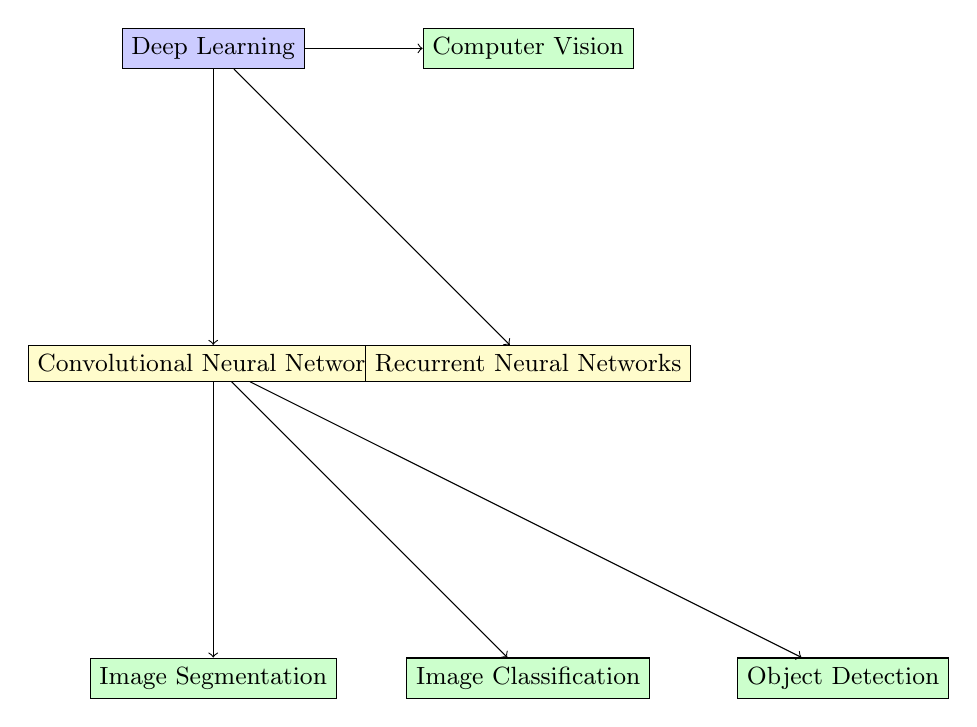
\begin{tikzpicture}[node distance=4cm]
        \tikzstyle{every node}=[font=\small]
        
        % Nodes
		\node (deeplearning) [rectangle, draw, fill=blue!20] {Deep Learning};
		\node (cv) [rectangle, draw, fill=green!20, right of=deeplearning] {Computer Vision};
		\node (cnn) [rectangle, draw, fill=yellow!20, below of=deeplearning] {Convolutional Neural Networks};
		\node (rnn) [rectangle, draw, fill=yellow!20, below of=cv] {Recurrent Neural Networks};
		\node (segmentation) [rectangle, draw, fill=green!20, below of=cnn] {Image Segmentation};
		\node (classification) [rectangle, draw, fill=green!20, right of=segmentation] {Image Classification};
		\node (detection) [rectangle, draw, fill=green!20, right of=classification] {Object Detection};
        
        % Edges
        \draw[->] (deeplearning) -- (cv);
        \draw[->] (deeplearning) -- (cnn);
        \draw[->] (deeplearning) -- (rnn);
        \draw[->] (cnn) -- (segmentation);
        \draw[->] (cnn) -- (classification);
        \draw[->] (cnn) -- (detection);
        
    \end{tikzpicture}
    \caption{Relationship between Deep Learning and Computer Vision}
\end{figure}


\subsection{主要挑战和进展}
计算机视觉作为一个快速发展的跨学科研究领域,长期以来一直面临着诸多关键挑战。其中最为核心的包括图像识别的准确性、对高维视觉数据的处理能力以及在复杂环境下的适应性等方面的困难。
首先,图像识别准确性的提升一直是计算机视觉领域的重点研究方向。由于不同环境、光照、角度等因素的变化会严重影响视觉对象的视觉特征,导致识别效果大幅下降。这直接制约了计算机视觉系统在复杂场景中的应用。
其次,视觉数据通常呈现出高维、大规模的特点,给数据处理和分析带来了巨大挑战。传统的特征工程方法已无法有效应对如此复杂的视觉数据,需要更加强大的计算能力和建模技术。
此外,计算机视觉系统还需要在复杂多变的环境中保持稳定和可靠的性能表现,这对系统的鲁棒性提出了较高要求。
幸运的是,随着深度学习技术的快速发展,这些挑战正在得到有效缓解。以卷积神经网络为代表的深度学习模型,在图像分类、物体检测等核心视觉任务上取得了突破性进展,大幅提升了计算机视觉系统的识别准确率。同时,这些模型也展现出强大的大规模数据处理能力,使得实时分析和理解大量视觉数据成为可能。
\subsection{应用领域的拓展}
计算机视觉技术的应用领域近年来呈现出快速扩张的趋势。最初,该技术主要应用于工业检测和医学影像分析等相对受控的场景中。但随着深度学习等先进算法的发展,计算机视觉的应用范围已经大幅拓展到了诸多新兴领域。

在智能驾驶领域,计算机视觉发挥着关键作用。通过对道路、障碍物、行人以及交通标志等视觉信息的实时检测和识别,自动驾驶系统可以准确感知周围环境,从而做出安全可靠的决策和控制。这不仅提高了行车安全性,还为实现完全自主驾驶奠定了基础。

在零售和广告领域,计算机视觉可以对消费者的面部表情、行为模式等进行分析,从而提供个性化的购物体验和广告内容。例如,通过分析消费者的目光焦点、情绪变化等,零售企业可以及时调整商品陈列和促销方案,提高销售转化率;广告公司也能根据受众的反馈优化广告内容和投放策略,提升广告效果。

此外,计算机视觉技术还广泛应用于智能监控、人脸识别、增强现实等领域。在智能监控中,该技术可以自动检测可疑行为,大大提高安全防控效率;在人脸识别中,它能够准确高效地完成身份验证和追踪;在增强现实领域,它则赋予AR/VR系统感知环境和交互的能力。

\sectionbreak

% ---------------------------------------------------------------------------- %
\section{机器学习与计算机视觉处理}
\subsection{机器学习}
机器学习是一种使计算机系统利用数据(或过往经
验)实现自我提升性能的方法论。机器学习主要分为3
类:监督学习、无监督学习和强化学习\textsuperscript{[1]}。
在监督学习中,算法从标记的训练数据中学习,以
预测新数据的输出。线性回归公式可以表示为
\begin{equation}
	y = wx + b
	\end{equation}
其中$\textit{y}$是预测值,$\textit{x}$是输入特征,$\textit{w}$和$\textit{b}$分别是模型的
权重和偏置。无监督学习处理未标记的数据,旨在发现
隐藏的数据模式,典型的无监督学习算法有K-means
聚类和主成分分析(PCA)\textsuperscript{[2]}。K-means聚类中,目
标是最小化每个点到其所属类中心的距离平方和,即
\begin{equation}
	J = \sum_{i=1}^{k} \sum_{x \in S_i} |x - \mu_i|^2
	\end{equation}
其中$u_i$是$S_i$簇的中心。强化学习
是一种学习如何在特定环境中采取行动以最大化某种累
积奖励的方法。强化学习中,价值函数通常用来估计在
状态下获取的预期回报
\subsection{计算机视觉处理}
计算机视觉是使机器“看”和“理解”世界的科学,
利用相机、计算机和算法来模拟和扩展人眼的视觉功
能,涵盖了从图像获取、处理到解释和理解的全过程。
图像处理的目的是改善图像数据或从图像中提取有
用信息,包括但不限于以下几个方面。
\begin{enumerate}
	\item 图像增强:提高图像的视觉效果,如对比度和亮度调整。
	\item 图像分割:将图像分割成多个部分或对象。
	\item 特征提取:识别和提取图像中的关键特征。
	\end{enumerate}
边缘检测用于识别图像中物体的边界,常用的算法
有Sobel、Canny等\textsuperscript{[3]}。Sobel算子用于边缘检测,其
核心计算可表示为
\begin{equation}
	G = \sqrt{G_x^2 + G_y^2}
	\end{equation}
其中$G_x^2$和$G_y^2$分别是图像在水平和垂直方向的梯度。
图像在水平和垂直方向的梯度;在不同图像之间寻找相
同特征,关键算法包括SIFT和SURF\textsuperscript{[4]};识别图像中
的特定对象,如使用深度学习模型。计算机视觉面临的
主要挑战包括光照变化、视角变化、遮挡问题等。
\subsection{计算机视觉处理中的机器学习应用}
\begin{enumerate}
	\item 图像分类:通过学习大量标注数据,模型能够
	识别和分类新图像中的主要内容。如今,深度神经网络
	在图像分类任务中已达到甚至超越人类水平。
	\item 目标检测:不仅识别图像中的对象,还需要确
	定其位置。这在监控、自动驾驶等领域有着重要应用。
	\item 语义分割:将图像分割成多个区域,并识别每个
	区域的类别。这对于理解场景的整体结构至关重要,例如
	在自动驾驶中理解道路、行人和障碍物的位置关系。
	\end{enumerate}
结合机器学习,特别是深度学习,计算机视觉已经
取得了飞速发展。卷积神经网络(CNN)是最突出的
例子,它在图像分类、目标检测等多个领域表现卓越。
卷积神经网络的卷积层可以表示为
\begin{equation}
	F(x) = \mathbf{W} * x + b
	\end{equation},其中*
表示卷积操作,$textit{x}$和$textit{b}$分别是卷积核的权重和偏置。循
环神经网络(RNN)和长短期记忆网络(LSTM)用于
处理视频或序列图像中的时序信息,它们通过记忆先前
的输入,在视频分析和事件预测中发挥重要作用。生成
对抗网络(GAN)由生成器和判别器组成,能够生成逼
真的图像,应用于图像生成、图像风格转换等领域。
深度学习技术使得面部识别在安全认证、个人识别
等领域得到广泛应用。机器学习特别是深度学习在自动
驾驶汽车中的应用,使得车辆能够实时处理和理解周围
环境,做出准确的驾驶决策

\sectionbreak

\section{主要应用策略}
\subsection{机器学习在艺术风格迁移中的应用}
艺术风格迁移首先选择目标内容图像和风格参考图像,使用预训练的 CNN(如 VGG 网络)从两幅图像中提取特征。内容通常由网络的浅层表示,而风格由深层表示,定义一个包含内容损失和风格损失的目标函数。
内容损失 $L_{content}$ 确保新图像与内容图像在内容上相似;
风格损失 $L_{style}$ 确保新图像与风格图像在风格上相似。整体损失函数如式 (4-1) 所示:
\begin{equation}
L_{total} = \alpha L_{content} + \beta L_{style}
\end{equation}
其中, $\alpha$ 和 $\beta$ 是调节两个损失影响的权重因子。
通过梯度下降算法最小化,从而生成具有目标风格的新图像。
\subsection{机器学习在图像内容定义中的应用}
图像内容定义,即从图像中识别和理解对象及场景,是计算机视觉的关键任务之一。随着机器学习,尤其是深度学习的发展,这一领域获得了显著发展。现代应用如医疗成像、自动驾驶等依赖于精确的图像内容定义。

对图像进行格式标准化,例如,大小调整公式可以表示为 resize$(I,w,h)$,其中 $I$ 是原始图像, $w$ 和 $h$ 是新的宽度和高度。用卷积神经网络 (CNN) 提取关键特征,CNN 特征提取可表示为 $F=\mathrm{CNN}(I)$,其中 $F$ 是提取的特征,$I$ 是输入图像。

应用分类模型识别图像内容,使用 Softmax 函数进行分类,公式为 $P(y|F)=\text{soft max}(W \cdot F+b)$,其中 $F$ 是给定特征 $P(y|F)$ 时类别 $y$ 的概率, $W$ 和 $b$ 是模型参数。

基于识别结果进行标记和汇总,使用非极大值抑制 (NMS) 处理重叠的检测框,公式为 $\mathrm{NMS}(B,\theta)$,其中 $B$ 是候选框集合, $\theta$ 是重叠阈值。
\subsection{机器学习在图像内容重构中的应用}
图像内容重构的典型过程如下。
\begin{enumerate}
	\item 图像预处理:这可能包括去除噪声、调整对比
	度等步骤。例如,可以使用高斯滤波器去除噪声,其公式 (4-2) 所示:
	\begin{equation}
	G(x, y) = \frac{1}{2\pi^2} e^{-\frac{x^2 + y^2}{2\sigma^2}}
	\end{equation}
	\item 特征提取:使用卷积神经网络 (CNN) 从图像中提取深层特征。类似于图像内容定义,特征提取如式 (4-3) 所示:
	\begin{equation}
	F = \mathrm{CNN}(I)
	\end{equation}
	\item 图像重构:应用深度学习模型,如生成对抗网络 (GAN),进行图像重构。
	\item 后处理:进一步优化重构图像,例如使用双三次插值进行上采样,其公式如式 (4-4) 所示:

	\begin{equation}
	B(x, y) = \sum_{i, j} f(i, j)h(x - i, y - j)
	\end{equation}
	
	其中 $h$ 是插值核。
\end{enumerate}

在医学成像领域,图像重构技术被用来增强图像的可读性,从而帮助医生进行更准确的诊断。另外,在数字影像修复领域,它可以用来恢复老旧或损坏的照片。机器学习在图像内容重构中的应用展示了其强大的图像处理能力。随着算法的不断进步,可以期待在更多领域看到高质量、高效率的图像重构应用。
\subsection{机器学习在图像风格定义中的应用}
图像风格定义是指利用机器学习技术分析和复现特
定图像的风格特征。这不仅包括艺术风格迁移,还涉及
图像风格的自动分类和识别。随着深度学习的发展,尤
其是卷积神经网络(CNN)在图像处理方面的应用,
图像风格定义已经成为了计算机视觉领域的一个热门研
究方向。
图像风格定义通常包括以下步骤。
\begin{enumerate}
	\item 图像预处理:与其他图像处理任务一样,首先
	需要对图像进行标准化处理,如调整尺寸、规范化颜色等。
	\item 特征提取:使用深度学习模型,如CNN,提取图像的高级特征。这些特征包括图像的纹理、颜色分
	布、形状等,对于风格识别至关重要。
	\item 风格分类/识别:训练机器学习模型对提取的
	特征进行分类或识别,以确定图像的风格。这可以通过
	分类算法实现,如支持向量机(SVM)或深度神经网络。
	\item 后处理:根据需要对分类或识别的结果进行后
	处理,如标记风格类型。
	\end{enumerate}
\hspace{2em}在艺术品分析中识别画家的风格,或在设计领域自动
分类不同的设计风格时,通过分析颜色、笔触和形状等特
征,机器学习模型可以区分毕加索和梵高的画作风格。
机器学习在图像风格定义中的应用不仅能够帮助人
们更好地理解和分析艺术作品,在广告、时尚和设计等
领域也具有广泛的应用前景。随着技术的进一步发展,
可以预见到更多创新应用的出现。
\sectionbreak

\section{结语}
本文综合考察了基于机器学习的计算机视觉应用,
深入探讨了其在多个子领域的发展和应用。从图像处理
到艺术风格迁移,从图像内容定义到图像重构,再到图
像风格定义,机器学习技术在计算机视觉中的应用表现
出了无限的潜力和广阔的应用前景。
\sectionbreak


% ----------------------------------- 参考文献 ----------------------------------- %
\begin{thebibliography}{4}
	[1] 沈一心. 基于机器学习的计算机视觉应用[J]. 电脑编程技巧与维护, 2023(8): 109-111.\newline

	[2] 杨朋波, 桑基韬, 张彪, 等. 面向图像分类的深度模型可解释性研究综述[J]. 软件学报, 2023, 34(1): 230-254.\newline

	[3] 朱飞, 张煦尧, 刘成林. 类别增量学习研究进展和性能评价[J]. 自动化学报, 2023, 49(3): 635-660.\newline

	[4] 李国瑞, 许鹏飞, 彭三城, 等. 基于张量奇异值分解的视觉域自适应方法[J]. 计算机学报, 2023, 46(10): 2084-2096.

\end{thebibliography}
% ------------------------------------ 附录 ------------------------------------ %
\clearpage
\appendix
\phantomsection
\addcontentsline{toc}{section}{附录}
\section*{附录}
\subsection*{高斯滤波器}
高斯滤波器是一种用于图像平滑和噪声抑制的常用滤波技术。它利用高斯函数作为卷积核,可以有效地消除图像中的高频噪声,同时保留图像的主要特征。
高斯滤波器的数学表达式如下:
$G(x,y) = \frac{1}{2\pi\sigma^2}e^{-\frac{x^2 + y^2}{2\sigma^2}}$
其中,$(x,y)$表示像素坐标,$\sigma$为高斯核的标准差,控制着滤波的强度。标准差越大,滤波效果越强,但同时也会使图像细节模糊程度增加。

高斯滤波器具有以下特点:
\begin{enumerate}
	\item 能够有效抑制高频噪声,平滑图像细节。
	\item 计算简单,实现方便,在图像处理中广泛应用。
	\item 可以通过调节标准差$\sigma$控制滤波强度,以平衡噪声抑制和细节保留。
	\item 高斯核具有旋转不变性,可以对图像进行各向同性的平滑处理。
	\end{enumerate}
\hspace{2em}总的来说,高斯滤波器是一种非常实用的图像平滑算法,在去噪、锐化、边缘检测等图像预处理任务中扮演着重要的角色。


\end{document}
